
% {\setbeamercolor{background canvas}{bg=red!15}

\begin{frame}[fragile]
\frametitle{Exercise: Structure}
Add the following lines to the preamble of your document. \\
\textit{\small Try to keep the preamble structured logically!}
\begin{alertblock}{Enabling Structure Control from the Preamble}
    \small
    \begin{minted}{latex}
    \usepackage{multicol}
    \usepackage{hyperref}
    % or \usepackage[hidelinks]{hyperref}
    
    \pagenumbering{arabic}
    \setlength{\columnsep}{1cm}

    \renewcommand*\contentsname{Summary}    
    \end{minted}
\end{alertblock}
\end{frame}


\begin{frame}[fragile]
\frametitle{Exercise: Structure} 
\begin{alertblock}{Add Content to Document Body}
    \small
    \begin{minted}{latex}
    \tableofcontents
    
    \section{Introduction} \label{sec:intro}
    In this article, I would like to enumerate for you 
    the ways in which \LaTeX{} is preferable to ``the 
    word processor who shall not be named."

    \subsection{User Interface}
    I haven't decided what to write yet.

    \section{A Brief History}
    In Section~\ref{sec:intro}, I said...
    \end{minted}
\end{alertblock}
\end{frame}


\begin{frame}[fragile]
\frametitle{Challenge: Structure}
\begin{center}
\textbf{Recreate the following document:} \\
\end{center}
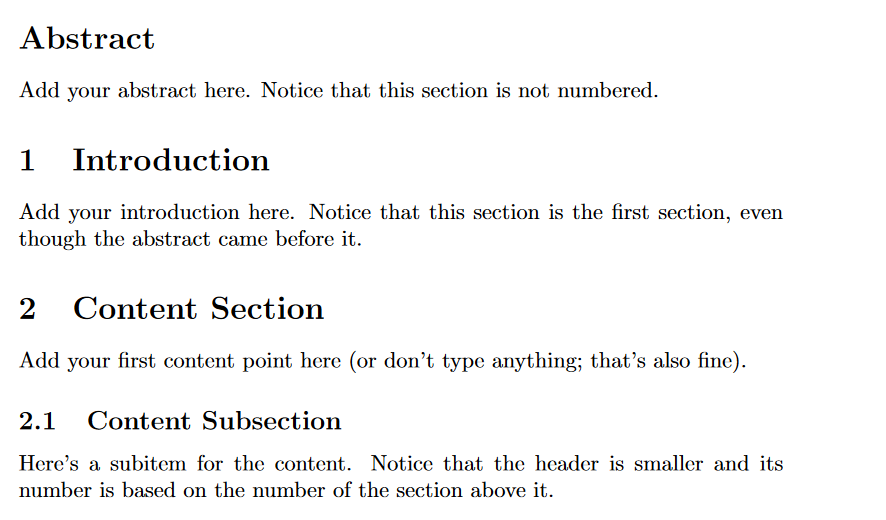
\includegraphics[width=0.9\linewidth]{img/structure_challenge.png}
\end{frame}


\begin{frame}[fragile]
\frametitle{Challenge: Structure}
\begin{alertblock}{Structure Source Code}
\small
\begin{minted}{latex}
\section*{Abstract}
Add your abstract here. 
Notice that this section is not numbered. 
\section{Introduction}
Add your introduction here. 
Notice that this section is the first section, even 
though the abstract came before it.
\section{Content Section}
Add your first content point here 
(or don't type anything; that's also fine).
\subsection{Content Subsection}
Here's a subitem for the content. 
Notice that the header is smaller and its number is 
based on the number of the section above it.
\end{minted}
\end{alertblock}    
\end{frame}


% \begin{frame}[fragile]
% \frametitle{Challenge: Cross-References}
% \begin{center}
%     \textbf{Recreate the following document: }\\
% \end{center}
% \vspace{0.2cm}
% 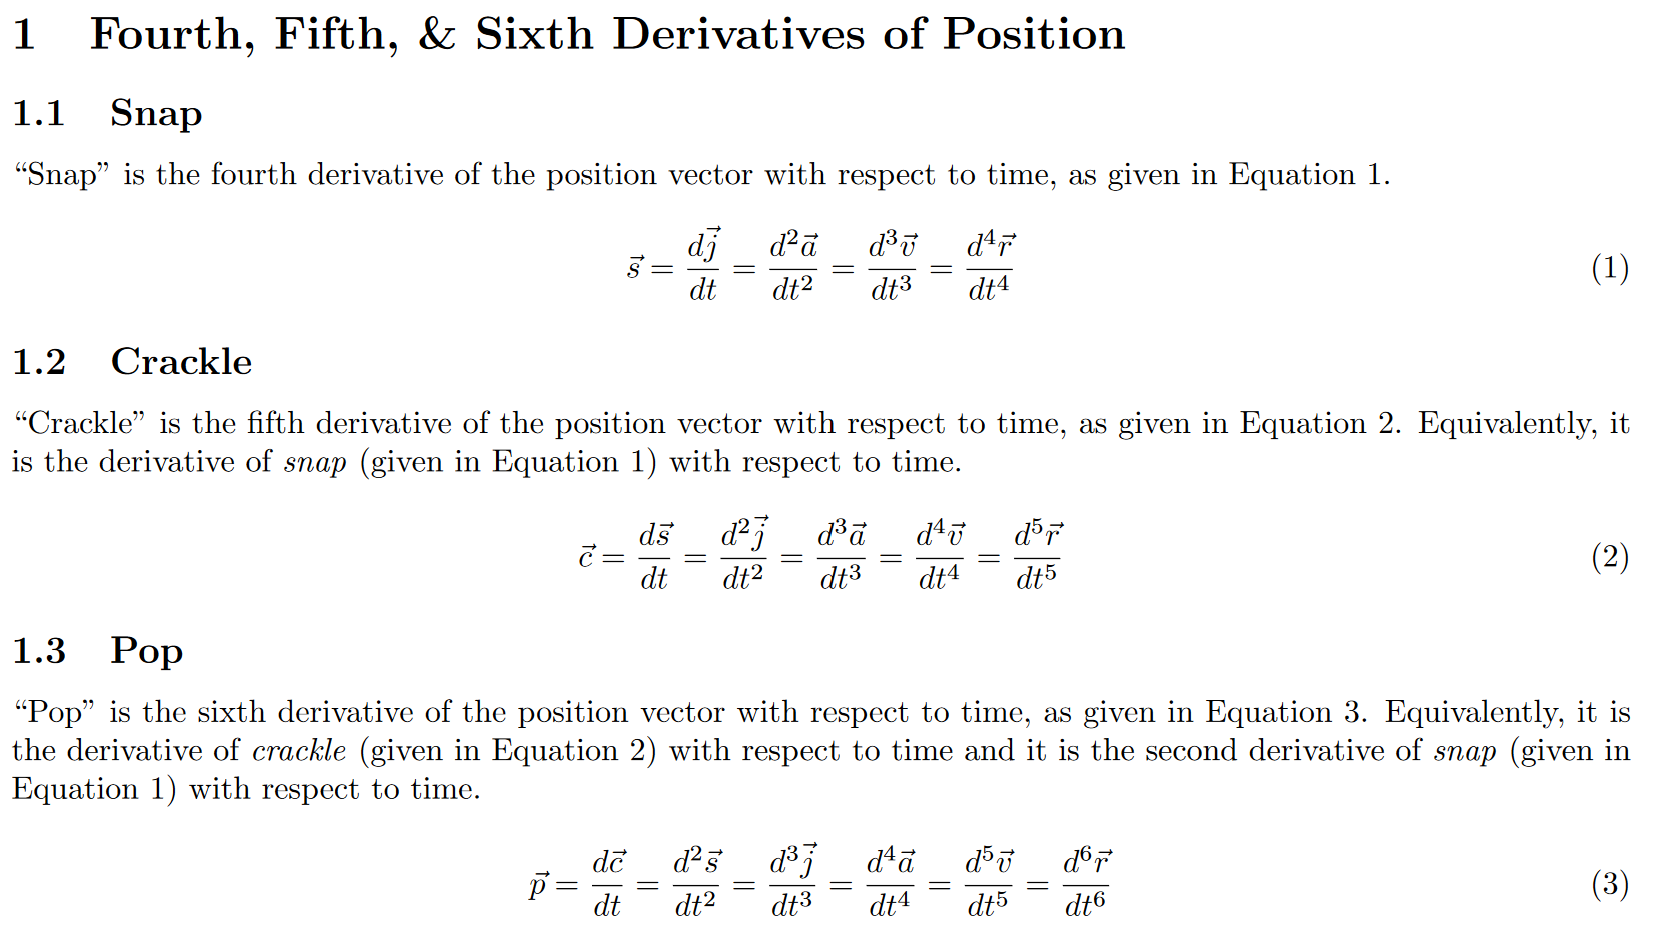
\includegraphics[width=\linewidth]{img/cereal.png}
% \end{frame}


% \begin{frame}[fragile]
% \frametitle{Challenge: Cross-References}
% \begin{alertblock}{Cross-References Source Code (1/3)}
% \small
% \begin{minted}{latex}
% \section{Fourth, Fifth, \& Sixth Derivatives of Position}

% \subsection{Snap} \label{sec:snap}

% ``Snap" is the fourth derivative of the position vector 
% with respect to time, as given in Equation~\ref{eq:snap}.

% \begin{equation} \label{eq:snap}
%     \Vec{s} 
%     = \frac{d\Vec{j}}{dt} = \frac{d^2 \Vec{a}}{dt^2} 
%     = \frac{d^3 \Vec{v}}{dt^3} = \frac{d^4 \Vec{r}}{dt^4}
% \end{equation}
% \end{minted}
% \end{alertblock} 
% \end{frame}




% }
